\documentclass[sagev, Crown]{sagej}

%\usepackage{algorithmic}
\usepackage{algorithm}
\usepackage{algorithmicx}
\usepackage{algpseudocode}
\usepackage{booktabs}
\usepackage{array}
\usepackage{graphicx}
\usepackage{amsmath}
\usepackage{amsfonts}
\usepackage{amssymb}
\usepackage{multirow}
\usepackage{url}

\setcounter{secnumdepth}{3} %Gives section numbers for cross referencing

\begin{document}

\runninghead{Wilson et al.}

\title{Robust, value-based sample size determination for clinical trials when nuisance parameters are unknown}

\author{Duncan T. Wilson\affilnum{1}}%,

\affiliation{\affilnum{1}Leeds Institute of Clinical Trials Research, University of Leeds, Leeds, UK} 

\corrauth{Duncan T. Wilson, Clinical Trials Research Unit, Leeds Institute of Clinical Trials Research, University of Leeds, Leeds, LS2 9JT, UK}
\email{d.t.wilson@leeds.ac.uk}

\begin{abstract}
% 200 word limit (250 for YSM)

\textbf{Background:} The conventional approach to determining the sample size of a clinical trial is to choose the smallest value such that the power of the trial is above a nominal threshold. This sample size can be highly sensitive to nuisance parameters, such as the variance of a continuous primary outcome. Moreover, this approach not formally account for the costs of sampling, and as a result can lead to incoherent decisions.

\textbf{Methods:} We present an alternative model for sample size determination which explicitly balances costs and benefits by introducing a value function to be maximised. We explore the implications of the model and argue it provides a better representation of sample size determination in practice than the conventional approach. We show the method is significantly less sensitive to nuisance parameters, to the point where a fixed design with no interim sample size adjustment can be near-optimal for large regions of the nuisance parameter space. We propose a criterion for choosing an optimal fixed sample size, considering the range of nuisance parameter values for which the value of the fixed design is within a tolerable distance of the value of the best possible design.

\textbf{Results:} We illustrate our approach by applying it to two trial design problems: choosing the accrual and follow-up times for a parallel group trial comparing overall survival, where the median survival time in the control arm is unknown; and choosing the number of clusters in a cluster randomised trial with unknown variance components at both the individual and cluster levels.

\textbf{Conclusion:} Accounting for the costs of sampling when determining the sample size of a clinical trial,  we can find simple, fixed sample size designs which are highly robust to nuisance parameter uncertainty.
\end{abstract}

\keywords{Clinical trials, sample size, power, interim analysis, internal pilot, sample size re-estimation}

\maketitle


\section{Introduction}\label{sec:intro}

When designing a clinical trial, the standard approach to sample size determination (SSD) is to choose the smallest sample size which will ensure that the power of the trial will be greater than a pre-specified nominal threshold (often 80 or 90\%). Power is defined in relation to a target effect size (specifically, the minimal clinically important difference \cite{Cook2018}), and under some modelling assumptions. These assumptions will typically include the value of one or more nuisance parameters in the model, and so these must be estimated prior to the trial. Incorrect estimates can lead to the actual power of the trial differing from the planned power. The greater the error in estimation, the greater the discrepancy between planned and actual power.

One approach to addressing uncertainty in nuisance parameter values is to conduct a small \emph{pilot} trial prior to the planned definitive study \cite{Browne1995, Gould2001, Friede2006}. The pilot data can then be used to estimate the nuisance parameter, with this estimate then being used in the sample size calculation of the definitive trial. This leads to the definitive trial sample size being a random variable (a function of the pilot trial estimate),  meaning a certain degree of precision in the pilot estimate is required to avoid excessive variability in the main trial sample size, and the cost of sampling in the pilot must be weigh

traded-off against the benefits it will bring \cite{Teare2014, Whitehead2015}. In some cases, such as in cluster randomised trials, sufficient precision is not attainable within the constraints of a pilot study \cite{Lake2002, Eldridge2015}. When the pilot will deliver a sufficiently  precise estimate, it may nevertheless be an undesirable procedure due to logistical reasons. For example, a long-term primary endpoint would cause significant delay to starting the definitive trial if it must first be measured in a pilot trial. Thus, pilot estimation may not always be the best way to address uncertainty in the nuisance parameter.

The conventional approach to SSD does not formally allow for the costs of sampling to be taken into account. Informally, this is often done through the so-called `sample size samba' \cite{Schulz2005}. This is the common procedure whereby the MCID declared for a study is iteratively adjusted until the sample size required for nominal power is considered feasible. This is not an option when using a pilot trial to estimate the nuisance parameter, as the MCID will have been declared prior to the estimate being obtained. This results in an incoherent procedure in the sense that a sample size calculation based on an estimate could lead to very different choices depending on whether the estimate came from a pilot or from some other external source. We would argue that a SSD procedure should lead to the same decision whenever the same inputs are used.

Motivated by these difficulties, we propose an alternative approach to SSD which explicitly accounts for both the benefits and costs of the trial. We do this through introducing a value function, a linear combination of the trial's power and its sample size, and choosing the sample size which maximises value. We will show that this simple value-based approach  leads to a coherent re-estimation procedure with good operating characteristics and, in many cases, can eliminate the need for re-estimation altogether by finding designs which are robust to uncertainty in nuisance parameters.

The remainder of this paper is organised as follows. Two motivating examples are introduced in Section \ref{sec:examples}. In Section \ref{sec:methods} we define the conventional method for SSD and introduce the value-based alternative. These are then applied to the motivating examples in Section \ref{sec:examples}. We consider some extensions to the basic method in Section \ref{sec:extensions}, before concluding with a discussion in Section \ref{sec:discussion}.

\section{Motivating examples}\label{sec:examples}

% Two examples where we can't get precise pilot estimates, and so would get hugely variable n under standard SSR.

% Do we need these for motivation? Clearer if we just introduce them as examples after themethods have been described. Just need to make the motivation clear in the intro, perhaps mentioning pilot cRCTs and the results and recoemmendations in \cite{Eldridge2015}.

\subsection{Cluster randomised trial}\label{sec:ex_cRCT}

Consider a cluster randomised trial, with $k$ clusters in each of two arms and $m$ participants in each cluster. The primary outcome of participant $i$ in cluster $j$ and arm $k$ is normally distributed:
\begin{align*}
y_{i,j,k} & \sim N(u_j, \sigma_w^2) \\
u_j & \sim N(\mu_k, \sigma_b^2).
\end{align*}
The primary analysis will compare the cluster means between the two arms in a $t$-test. The nuisance parameter in this test is the variance of cluster means:
$$
Var(u_j) = \sigma_b^2 + \frac{\sigma_w^2}{m} = \sigma^2.
$$
Estimation of $\sigma^2$ (or equivalently, of the total variance and the ICC) is challenging due to the very small sample size, since the unit of measurement is the cluster. In a methodology study of external pilot cluster randomised trials, the sampling variability of pilot estimates was found to be so large that for a pilot to obtain a sufficiently precise estimate, the pilot sample size often needed to be as large as that of the definitive trial \cite{Eldridge2015}. This led the authors to conclude that sample size re-estimation is not feasible for cluster RCTs, and that nuisance parameter estimates should instead be sought from elsewhere.

% Add some specific numbers to illustrate how variable the definitive n can be?

\subsection{Closed cohort stepped wedge trial}\label{sec:ex_SW}

Consider a stepped wedge trial in five steps, or arms. In arm $i$, $k$ clusters start the trial in the control condition before adopting the intervention at time $j = i$. Each cluster is measured at each time point $j = 0, 1, \ldots , 5$. Measurement is at the individual level, with $m$ individuals in each cluster. The same individuals area measured at each time point, in what is known as a closed cohort stepped wedge design.

The suggested statistical model of this trial involves four nuisance parameters, each of which help determine power \cite{Hooper2016}. These parameters are:
\begin{itemize}
\item $\sigma^2$, the total variance;
\item $\rho$, the intracluster correlation;
\item $\pi$, the cluster autocorrelation; and
\item $\tau$, the individual autocorrelation.
\end{itemize}

We consider the `Girls on the Go!' trial as an example, taking the initial design, estimates of nuisance parameters, and MCID as \cite{Hooper2016}. There, a cluster size of $m = 10$ was assumed fixed and the constrained method gave an optimal number of clusters of $k = 4$, leading to a total sample size of 120 (due to the three arms of the stepped wedge design). Here, we will instead fix the number of clusters at $k = 4$, and consider varying $m$. The closed cohort nature of the design means that an internal pilot is not an option, as all individuals and clusters are recruited at the outset. An external pilot, while possible, might be expected to yield imprecise estimates if it is to be considerably smaller than the definitive trial. We will, therefore, not consider re-estimation in this example, focussing instead on finding a fixed design which is robust to uncertainty in the four nuisance parameters.

\section{Methods}\label{sec:methods}

We consider the choice of sample size for a trial aiming to estimate some parameter of interest, $\mu$, and test the null hypothesis $H_0: \mu = 0$ with a significance level $\alpha$ against an alternative hypotheses $H_1: \mu = \mu_1$. We denote the nuisance parameter by $\sigma$, its estimate by $\hat{\sigma}$, and the sample size by $n$. Both $\sigma$ and $n$ may be vectors. We denote the power of the trial by $\beta(n, \mu, \sigma)$, assuming from herein that $\alpha = 0.05$ (two-sided). We assume that, all other things being equal, a higher powered trial is preferred to a lower powered trial, and a trial of smaller sample size is preferred to a larger one. 

\subsection{Constrained design}

% Keep simple - one method is to get an estimate and use this under the contrained approach.
% Numerous variants, such as inflating the estimate, improsing upper and/or lower caps on the definitive n, adjusting the definitive n to avoid bias. For simplicity, focus on the basic method.

The conventional approach to sample size determination sets a constraint on the trial's power and finds
\begin{equation}
n^*_c (\mu_1, \hat{\sigma}, \beta^*) = {\arg\min}_{n \in \mathbb{N}}~ n ~\text{ subject to } ~ \beta(n, \mu_1, \hat{\sigma}) \leq \beta^*.
\end{equation}
The chosen sample size $n^*_c$ depends on the target difference $\mu_1$, the estimated nuisance parameter $\hat{\sigma}$, and the nominal type II error rate $\beta^*$. Although originally intended to be set at a level appropriate to the specific context \cite{}, a convention of arbitrarily setting $\beta^* = 0.2$ or 0.1 has emerged \cite{Bacchetti2019}. When $n^*_c$ is found to be infeasibly large, it is common to inflate the target difference $\mu_1$ from the true MCID to a higher value and thus reduce the required sample size \cite{Schulz2005}.

When $\mu_1$ and $\beta^*$ are fixed, the sample size is a function of the estimated nuisance parameter only. When there is uncertainty in this estimate, it has been recommended that it be inflated to guard against choosing a sample size which is too low (in the sense of leading to a power less than the nominal level). For example, when the estimate $\hat{\sigma}$ has a confidence interval around it, the upper end of that interval may be used instead \cite{Browne1995, Teare2014, Whitehead2015}. This approach is justified as being `conservative' in the sense that it will likely lead to a trial with power greater than the nominal rate, since $n^*_c$ is strictly increasing in $\hat{\sigma}$. 

\subsection{Value-based design}

% Need to add a fixed cost to the value function, so that we eventually decide to abandon the trial if the sd is too large.
% Elicit this by using our hypothetical power curve and choosing the n where we become indifferent between that n (and corresponding power) and not running the trial at all. 
% Gives a consistency check - can plot the region where value is <= 0, and this should include the point n = 0.
% So now, if the whole power curve is in the region of v <= 0 then we don't want to do the trial.
% Assume pilot fixed costs are 0, which is conservative in the sense that the argument for a simple fixed design will be stronger (and pragmatic since we will often run the pilot anyway for feasibility reasons so we effectively have it for free).

An alternative approach to SSD is to choose the point which maximises a \emph{value} function $v(n, \beta): \mathbb{N} \times [0,1] \rightarrow \mathbb{R}$ which describes our preferences between all possible pairs of sample size and type II error. Specifically, $v$ is such that
$$
(n, \beta) \text{ is preferred to }(n', \beta') \Leftrightarrow v(n, \beta) > v(n', \beta').
$$
That such a function exists follows from some decision-theoretic axioms \cite{French2000}. Regarding the specific functional form, we can safely assume that for any fixed $\beta$, $v_(n, \beta)$ as a function of $n$ and of $\beta$ will be strictly decreasing. We further assume that it will also be linear in each of these terms. That is, we assume the cost of increasing the sample size by some amount $\Delta$ is independent of the starting point $(n, \beta)$, and similarly for $\beta$. The value function will then be of the form
$$
v(n, \beta) = (1 - \beta) - \lambda n.
$$
We can now define the optimal sample size as
\begin{equation}
n^*_v (\mu_1, \hat{\sigma}, \lambda) = {\arg\min}_{n \in \mathbb{N}} ~ (1 - \beta(n, \mu_1, \hat{\sigma})) - \lambda n.
\end{equation}
This optimal sample size now depends on the parameter $\lambda$ in addition to the MCID $\mu_1$ and estimated nuisance parameter $\hat{\sigma}$. A convenient way to determine $\lambda$ is to plot power as a function of sample size, for some hypothetical $\hat{\sigma}$, and determine the point which best balances the two factors. The gradient of the power curve at this point is equal to $\lambda$. This is illustrated in Figure \ref{fig:p_curves}, where we plot power curves for a two-sample $t$-test and two values of the nuisance parameter, the outcome standard deviation. 

\begin{figure}
\centering
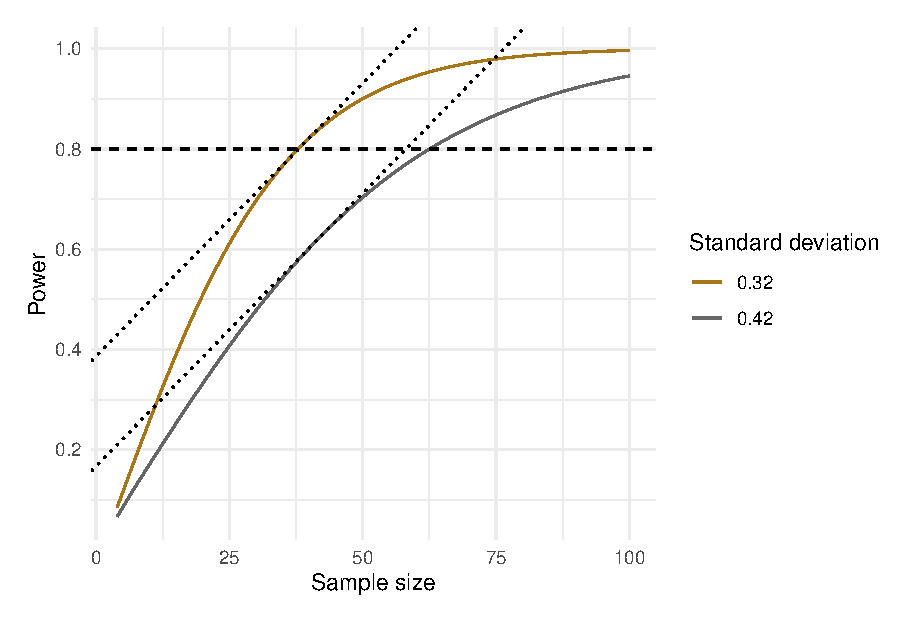
\includegraphics[scale=0.8]{./figures/p_curves}
\caption{Power curves for a two-sample $t$-test, for two values of the standard deviation of the outcome. The dotted lines indicate the rate at which power and sample size can be traded off with each other. The points where they are tangential to the power curves are the optimal value-based sample sizes.}
\label{fig:p_curves}
\end{figure}

\subsection{Eliciting $\lambda$}

We design the trial as normal using some fixed nuisance parameter, and allowing a samba, then read of the gradient at the corresponding point. It would be interesting to know how optimal designs vary as we vary the MCID we have in mind. So, graph lambda against a range of standardised effect sizes, when constraining to 80 or 90\% power.

\subsection{Uncertain $\sigma$}

- As well as fixed design, also introduce an SSR approach

Unlike the constrained method, $n^*_v$ is no longer monotonic increasing in $\hat{\sigma}$. When faced with uncertainty in $\sigma$, it is therefore no longer viable to simply inflate the estimate  $\hat{\sigma}$ on conservative ground. Denote a fixed design sample size by $n_f$. The optimal value-based sample size is a function of the nuisance parameter, denoted $n^*_v(\sigma)$. Then, for any $\sigma$, we can calculate the difference in value between the fixed and optimal designs:
$$
\delta(\sigma | n_f) = v[n^*_v(\sigma)] - v(n_f).
$$
We can choose a fixed design by maximising the area of nuisance parameter space $\Sigma$ over which the discrepancy $\delta(\sigma | n_f)$ is within some tolerable amount, $\delta^*$. That is, we solve
$$
n^*_f (\mu_1, \Sigma, \delta^*) = \arg\max_{n \in \mathbb{N}} \int_{\Sigma} I[\delta(\sigma | n) \leq \delta^*] d\sigma.
$$
We can use a Monte Carlo approximation, generating a set of nuisance parameter samples $\sigma^{(i)}, i = 1, \ldots , N$ from the uniform distribution over $\Sigma$. This then gives
\begin{equation}\label{eqn:fix}
n^*_f (\mu_1, \Sigma, \delta^*) = \arg\max_{n \in \mathbb{N}} \sum_{i=1}^N I[\delta(\sigma^{(i)} | n) \leq \delta^*].
\end{equation}

\section{Application to the examples}\label{sec:application}

\subsection{Cluster randomised trial}

To apply the value-based approach to the cluster RCT example of \ref{sec:ex_cRCT}, we note that the fixed cluster size was $m = 18$ and the best estimates of total variance and the ICC were 1 and 0.05, respectively. These give an initial estimate of the nuisance parameter of $\hat{\sigma} = 0.32$. The MCID is $\mu_1 = 0.3$. We suppose that the trade-off parameter is $\lambda = 0.01089517$. As illustrated in Figure \ref{fig:p_curves}, for  $\sigma = 0.32$ the value-based and constrained (using $\beta^* = 0.2$) methods agree, giving $ k = 37.87$ clusters.

Optimal sample sizes for both methods over a range of $\sigma$ values are illustrated in Figure \ref{fig:opt_t_test}. We see that the value-based sample size increases with $\sigma_c$, reaches a maximum, and then rapidly decreases. So, there is a point where the imprecision of measurement becomes too great to justify sampling. This can be contrasted with the constrained approach, where the sample size increases indefinitely with $\sigma$.

\begin{figure}
\centering
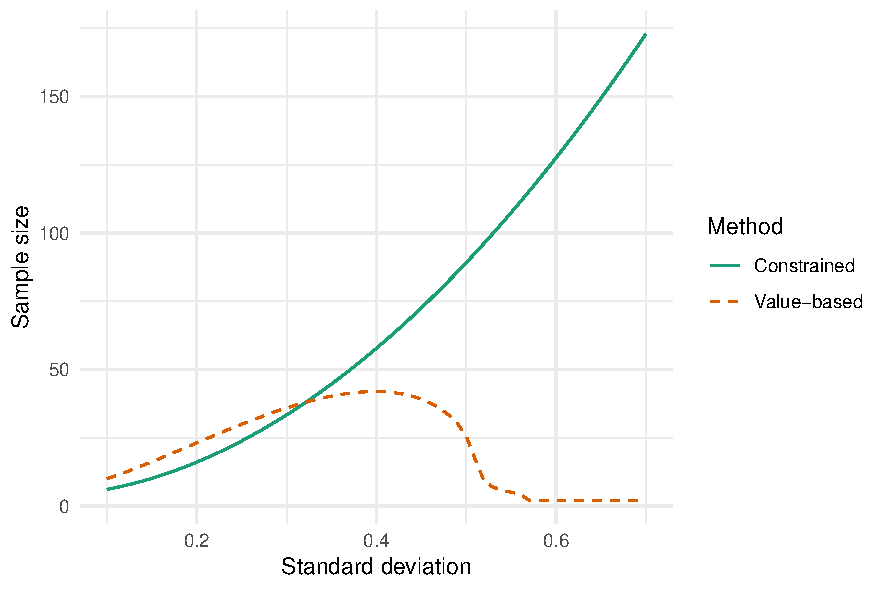
\includegraphics[scale=0.8]{./figures/opt_t_test}
\caption{Optimal sample size as a function of the standard deviation according to the constrained and value-based methods.}
\label{fig:opt_t_test}
\end{figure}

We examined using both methods in a re-estimation context. For three different values of the nuisance parameter, we simulated pilot estimates based on a pilot sample size of $k_p = 6$ clusters in total. Specifically, we sampled $10^3$ variates $\hat{\sigma}_j^{2 (i)} \sim \frac{\sigma^2}{k_p-1} \chi^2_{k_p-1}$ for both arms $j=1,2$ and $i = 1, 2, \ldots , 10^3$. The pooled sample standard deviation was then calculated as 
$$
\hat{\sigma}^{(i)} = \sqrt{\frac{(k_p - 1)\hat{\sigma}_1^{2 (i)} + (k_p - 1)\hat{\sigma}_2^{2 (i)}}{2k_p - 2}}.
$$
For each $\hat{\sigma}^{(i)}$ we re-estimated the definitive trial sample size using both the constrained and value-based methods. The distributions of the resulting sample sizes and corresponding powers are illustrated in Figure \ref{fig:dists_t_test}. We find considerably less variability in sample size when using the value-based method, particularly when the nuisance parameter has been under-estimated. The constrained method leads to essentially identical power distributions for all true nuisance parameter values, with an average power slightly below the nominal 80\% as a result of the small sample bias in the corrected sample standard deviations.

% Note that in this case (normal enpoint, estimating an sd) we can use the sample size formula given in \cite{Julious2006}, which gives a larger n based on the pilot estimate than the usual formula and as a result an expected power of the nominal level. These adjusted ns are a linear transformation of the standard ns, giving a larger variance in n. Should we use this, or just bring it up in the discussion? 

\begin{figure}
\centering
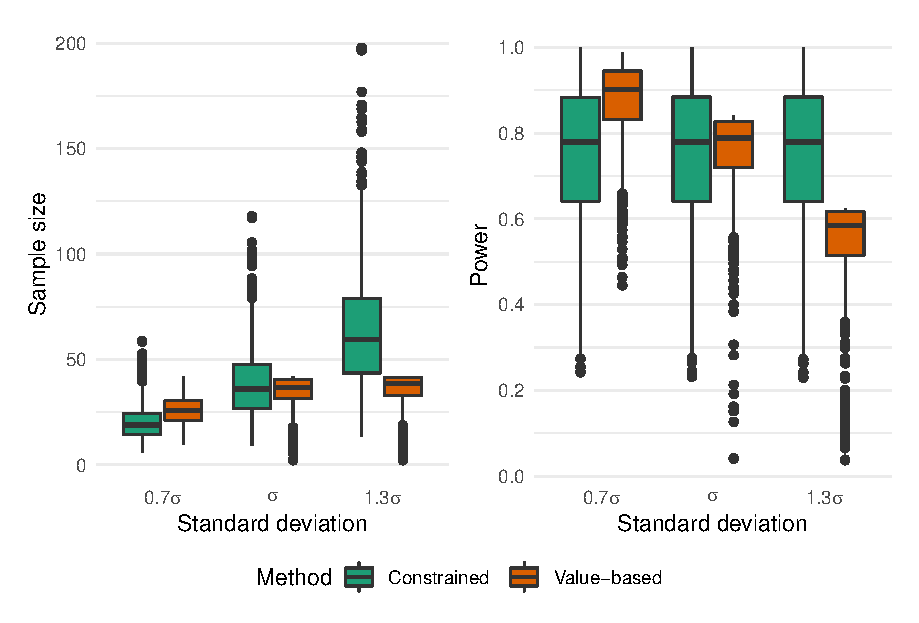
\includegraphics[scale=0.8]{./figures/dists_t_test}
\caption{Distributions of definitive trial sample size and power when re-estimating using the constrained and value based method, for true nuisance parameters based on $\sigma_c = 0.32$.  Boxplots show the median, first and third quartiles (hinges), and 1.5 $\times$ the inter- quartile range (whiskers).}
\label{fig:dists_t_test}
\end{figure}


To determine an optimal fixed design using the criteria of Equation (\ref{eqn:fix}), we set $\Delta = 0.03$. This gave an optimal fixed design with a total sample size of $n = 29$. The value of this fixed design as a function of $\sigma_c$ is plotted in Figure \ref{fig:fixed_t_test}, along with the value of the locally optimal design and the difference in value between the two. This shows that the fixed design is within $\Delta = 0.03$ of the locally optimal design for $\sigma_c \in [0.2, 0.54]$ (recall the initial estimate was $\sigma_c = 0.32$). If it is believed that this range will contain the true value, using this fixed design will not lead to much value being sacrificed and could lead to a more manageable, predictable, and feasible trial.

\begin{figure}
\centering
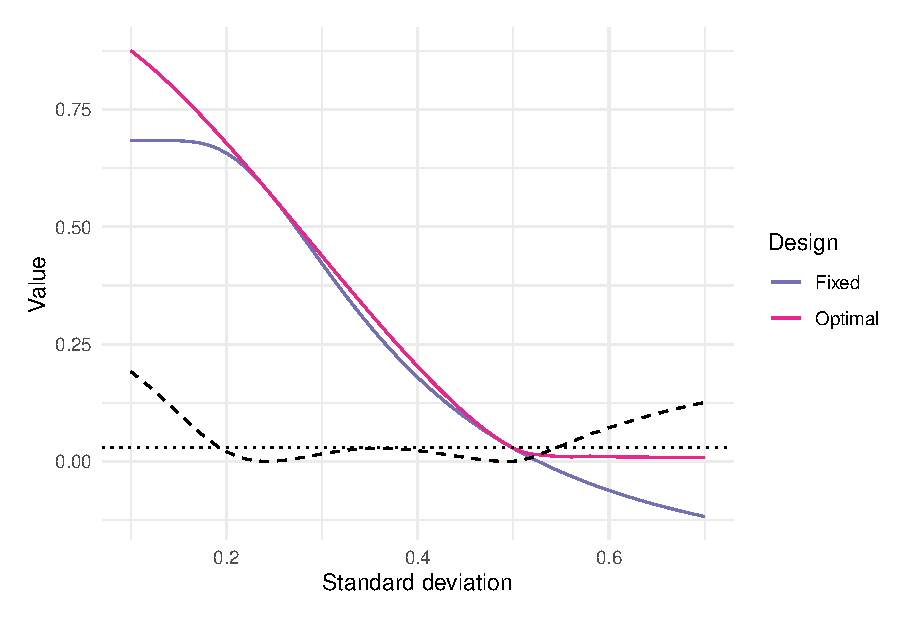
\includegraphics[scale=0.8]{./figures/fixed_t_test}
\caption{.}
\label{fig:fixed_t_test}
\end{figure}

\subsection{Closed-cohort stepped wedge trial}

Using the initial nuisance parameter estimates and the suggested optimal design of $k = 4$, we arrive at a trade-off parameter of $\lambda = 0.02502398$.

\begin{figure}
\centering
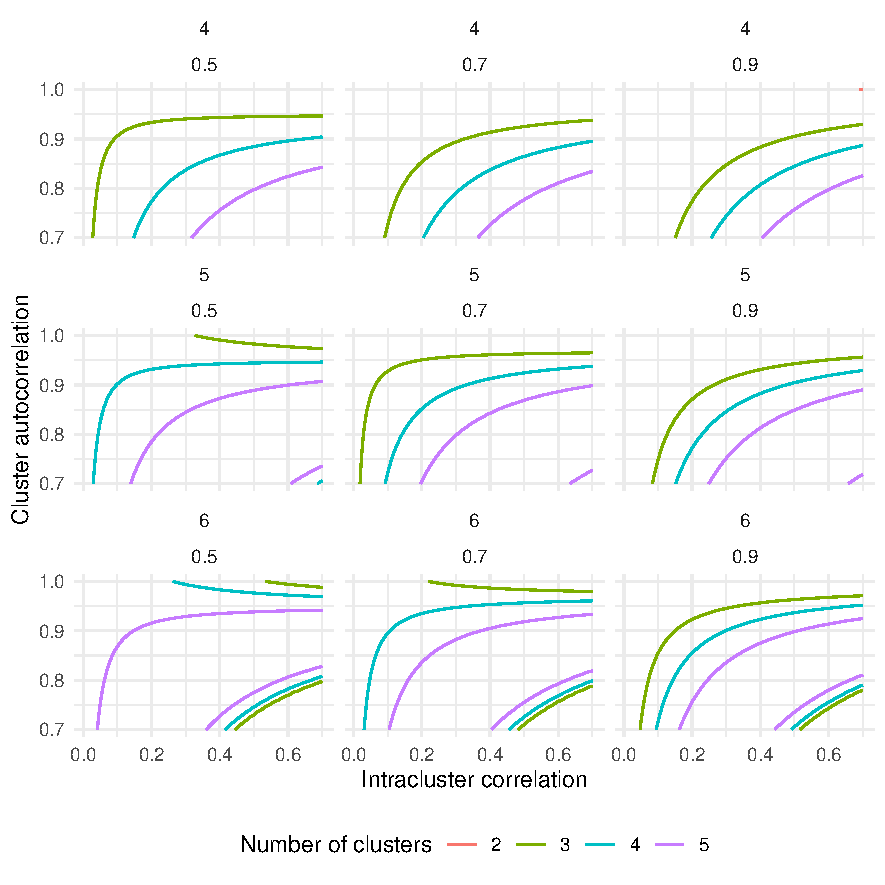
\includegraphics[scale=0.8]{./figures/opt_sw_k}
\caption{Optimal number of stepped wedge clusters for a range of true nuisance parameter values. Plots vary horizontally with the individual autocorrelation $\tau$, and vertically with the total variance $\sigma^2$.}
\label{fig:fixed_sw}
\end{figure}

\begin{figure}
\centering
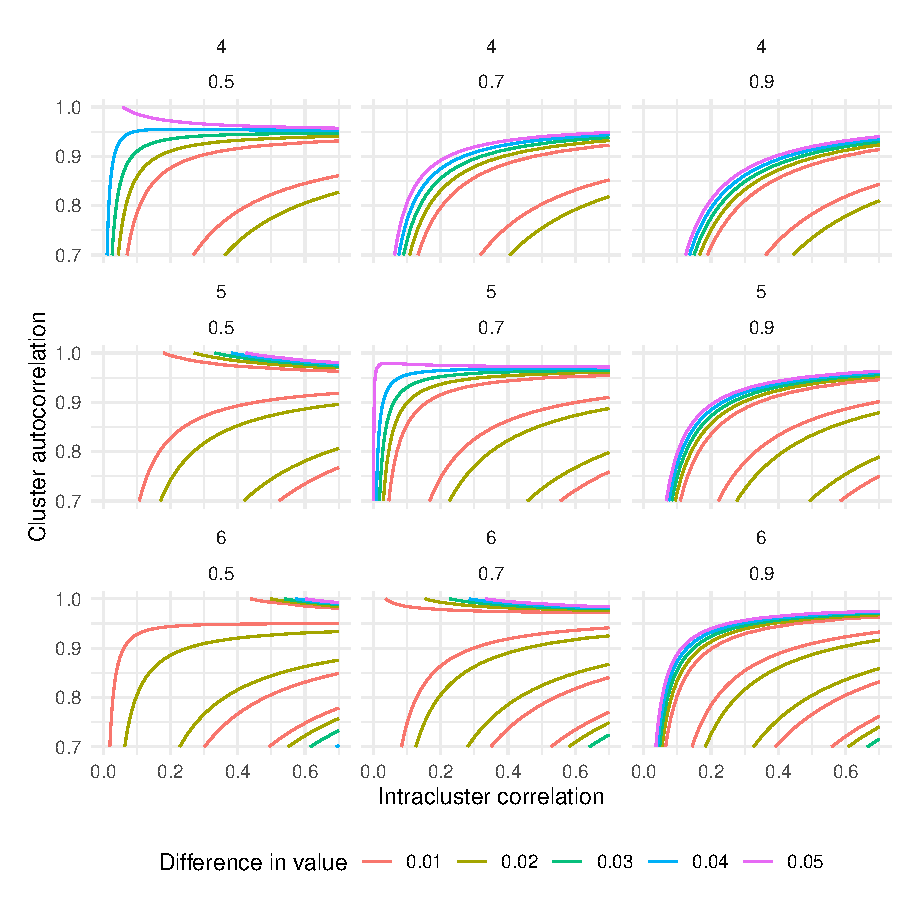
\includegraphics[scale=0.8]{./figures/fixed_sw_k}
\caption{Difference in value between fixed and locally optimal stepped wedge designs. Plots vary horizontally with the individual autocorrelation $\tau$, and vertically with the total variance $\sigma^2$.}
\label{fig:fixed_sw}
\end{figure}

\section{Evaluation}

In example 1 we showed that the re-estimated designs are quite different when using constrained or value based methods, but did not comment on their value - assuming that the value method will be better in this respect. In both examples we showed that a fixed design can be quite robust, i.e. that there would be little benefit to be gained from even a perfect re-estimation routine. 

We could extend our analyses by considering the admissibility of these decision rules. Admissable means that, for a given loss function, there is no other rule which is at least as good across the whole parameter space, and better in at least one part, in terms of its risk
$$
E_{x | \theta}[L(\theta, \delta(x))].
$$
Now, every admissible rule is a Bayes rule w.r.t. some prior $p(\theta)$, i.e. a rule which minimises the Bayes risk
$$
E_{\theta}[ E_{x | \theta}[L(\theta, \delta(x))] ] = E_{\theta, x}[L(\theta, \delta(x))].
$$
But every Bayes rule is also a generalised Bayes rule, i.e. a rule which will always minimise the posterior loss upon seeing $x$:
$$
E_{\theta | x} [L(\theta, \delta(x))].
$$
Now, we can see that any fixed design will be a generalised Bayes rule by choosing a degenerate prior which gives probability 1 to the point where that fixed design is optimal. So, any fixed design is admissible. 

Can we say something similar about the value rule? That is, is there a prior s.t. using that rule would be equivalent to minimising the posterior loss?

We may not be able to show that the value rule is admissible, but we can show that it dominates the constrained rule for the linear value function we have considered. The question is then, does there exist a value/loss function s.t. the constrained approach is admissible? 

\section{Extensions}\label{sec:extensions}

\subsection{Re-estimation in internal pilots}

All our arguments and methods hold in the internal pilot setting, where we re-estimate sample size after getting an interim nuisance parameter estimate. The complication is that type I error rate can be inflated, but many papers have identified how to correct for this in a variety of settings, including the t-test setting of our first example. Note that re-estimation is not possible in the second example.

The key difference between internal and external pilots is cost. For internal pilots, the sampling is "free" but there will be a penalty in terms of inflated alpha. So, might be easiest to cover both in the same general framework, where the internal pilot sampling cost term is calculated as the required inflation.

\subsection{Multiple design parameters}

For clarity, we have focussed on problems with a single design parameter, the sample size $n$. The value-based method extends naturally to a vector of design parameters. For example, a cluster RCT may allow for a choice of both the number of clusters $k$, the cluster size $m$, and the nominal type I error rate $\alpha^*$. If value is considered linear in all design parameters, and the power of the trial is convex, the trade-off parameters can be determined as in the single parameter case by choosing a design based on a hypothetical $\sigma$ and calculating the gradient of the power function, in terms of each design parameter dimension, at these points.

For example, returning to the cluster RCT example in Section \ref{sec:ex_cRCT}, we now consider choosing $k$ and $m$. Trade-off parameters are determined based on choosing the same design as before for the estimated nuisance parameter $\sigma_c = 0.32$ (that is, a locally optimal design of $k =19, m=18, n=342$ per arm). Note that we now need both the total variance and the ICC to calculate power, and so have two nuisance parameters: $\sigma_T^2$ and $\rho$. Searching for a robust fixed design as in \ref{} leads to a choice of $k = 16, m = 18, n = 288$ per arm. This was based on a nuisance parameter space where $\sigma_t^2 \in [0.1, 1.5]$ and $\rho \in [0.025, 0.1]$. The difference in value between the fixed and locally optimal designs over this space is illustrated in Figure \ref{} Over this space, the fixed design is within $\Delta = 0.03$ value units of the locally optimal design in approximately 99\% of cases. The only region of the subspace where this difference was exceeded was for small values of both $\sigma_t^2$ and $\rho$.

\begin{figure}
\centering
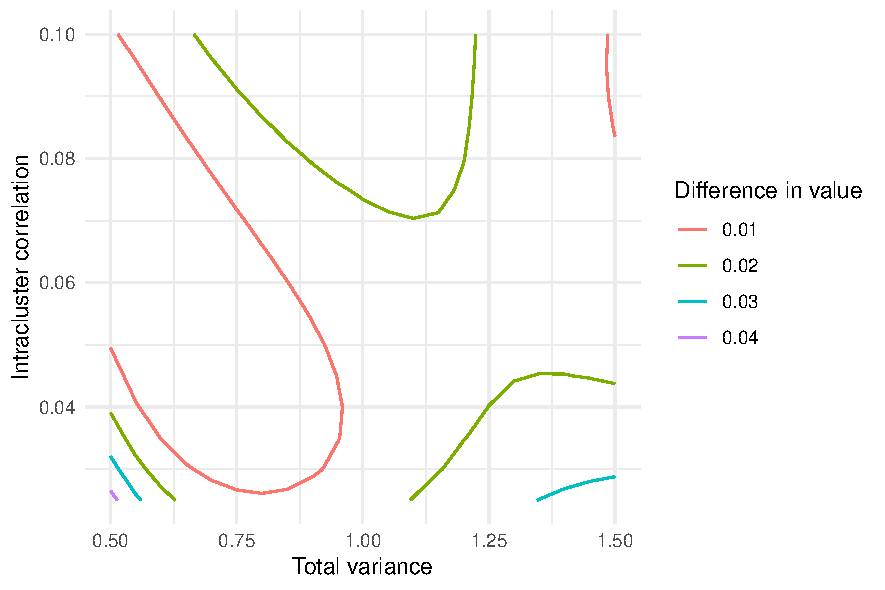
\includegraphics[scale=0.8]{./figures/mult_design}
\caption{Difference in value between fixed and locally optimal cluster randomised designs where both number of clusters and cluster size can be varied.}
\label{fig:mult_design}
\end{figure}

Extending to different sample size components would be simple enough in terms of the value function, using the same arguments of linearity and value additivity. Computationally, it might not be much worse - key thing is the number of discrete designs to evaluate. In the t-test example we have 1000. Can always argue for a coarser scale.

Key extension should be to cRCTs, either with control over m and k and two nuisnace params, over random m and control over only k, with four nuisance params. Note the latter will be fast, as only a few possible k options. But in both cases, SSR via integration over the sampling dist will be tricky and probably need MC. But it would be useful to show exactly how much more cumbersome the method becomes. Do both versions, include one in the paper and the other as SM. Also, start this extension noting that the t-test example covers cRCTs with fixed cluster size. 

Including alpha could be trickier, in terms of the value function. But this can go in discussion about extending to uncertainty in effect and the BAyesain conclusion, see below.

\subsection{Minimax optimality criterion}

An alternative optimality criteria for a fixed design is
$$
\min_{n \in \mathbb{N}} ~ \left[ \max_{\sigma \in \Sigma} ~  \delta(\sigma | n) \right].
$$
That is, we could choose the sample size with the smallest worst-case difference in value compared with the locally optimal design, over some range $\Sigma$. This criteria will be more sensitive to the choice of $\Sigma$; but it provides a way to better incorporate prior belief regarding likely values. As an example, using this criteria in the cluster RCT example of Section \ref{sec:ex_cRCT} and with $\Sigma = [0.22, 0.42]$ leads to a slightly larger fixed design of $n = 32$. The value of this design is plotted in Figure \ref{fig:minimax_t_test}.

\begin{figure}
\centering
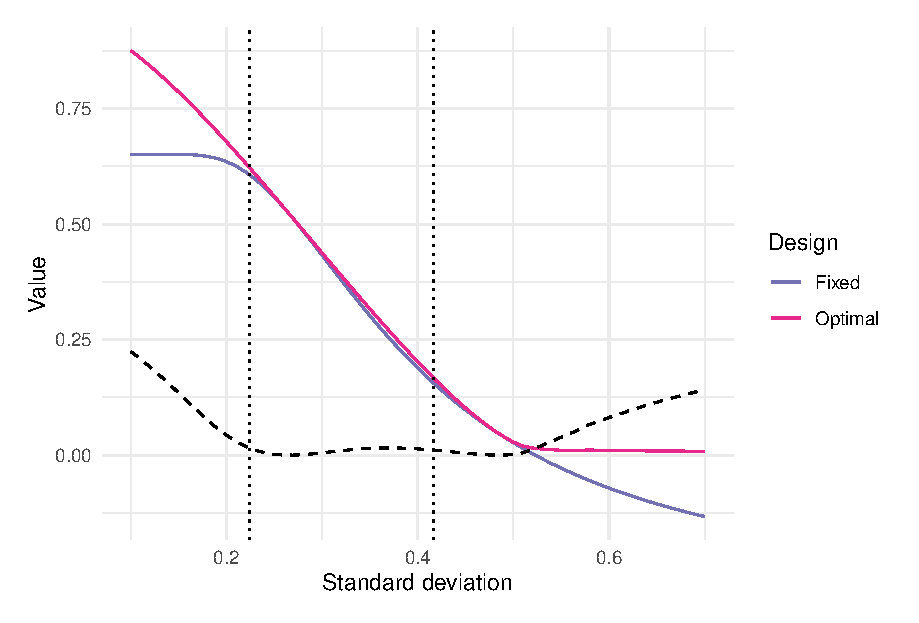
\includegraphics[scale=0.8]{./figures/minimax_t_test}
\caption{.}
\label{fig:minimax_t_test}
\end{figure}

This isa actually what we end up using, minimax regret. So put the other criteria here?

\subsection{Multi-criteria / efficacy}

We have focussed on trading off sampling with power at a specific point. We could argue that we are interested in power across the full (plausable) parameter space. If we had a discrete set of power points, we would start by combining into a weighted sum with weights reflecting the value at each point. The continuous analouge would be integrating the power function with some weighting function. This function would have to integrate to 1, so would be mathematically equivalent to a probability distribution. So this view would end up equivalent to a Bayesian analysis, where we maximise expected utility. But the latter would be easier in practice, as it separates out belief and value when eliciting the weighting function.

This encompasses the point of including alpha, so roll these points together.

\cite{Lin2004} - a phase II design which sets two alternative hypotheses, with different power constraints on each.

\cite{Kim2017} - extends to three hypotheses

\subsection{Simulation-based power}

Potentially another paper - for complex designs where we need MC for power calcs, could propose an alternative scalarising method as opposed to Pareto approach of WP4.1. Could use Laura's or Isabelle's problems as examples and collaborate? With a one-dimension value function to maximise over a several-dimension design space, we have the standard stochastic EGO approach (although note DICEoptim no longer on CRAN). Could extend to minimax regret SSD, which might be a bit more interesting / novel. This addresses the point in WP4.1. discussion that everything was conditional on estimates, but these might not be known, and we could model over the parameter space too. 

We would then want to choose, at each iteration, the design and point in the parameter space at which to simulate. We need to anticipate the improvement that evaluation will lead to. 

\section{Discussion}\label{sec:discussion}

The threshold myth, and how it would justify the constrained model but is a myth.

Incoherence in the standard SSD/R procedure resulting from the thereshold myth and ignorning costs.

Sample size samba in SSD, and note how this is impossible when doing SSR.

Ethics of underpowered and overpowered studies.

\cite{Schulz2005} - Sample size calculations in randomised trials: mandatory and mystical

\cite{Halpern2002} - The continuing unethical conduct of underpowered clinical trials

\cite{Lilford2002} - The Ethics of Underpowered Clinical Trials

\cite{Bacchetti2005a} - Ethics and sample size

\cite{Bacchetti2005} - Bacchetti et al. Respond to ``Ethics and sample size - Another view''

\cite{Norman2012} - Sample size calculations: should the emperor's clothes be off the peg or made to measure?

\cite{Edwards1997} - Why "underpowered" trials are not necessarily unethical

\cite{Girling2007} - Sample-size calculations for trials that inform individual treatment decisions: a 'true-choice' approach

\cite{Claxton1999} - The irrelevance of inference: a decision-making approach to the stochastic evaluation of health care technologies

\cite{Grayling2018} - Blinded and unblinded sample size reestimation procedures for stepped-wedge cluster randomized trial

\cite{Altman1980} - Statistics And Ethics In Medical Research: III How Large A Sample?

\cite{DeMartini2010} - Conservative Sample Size Estimation in Nonparametrics

\cite{Bacchetti2019} - The other arbitrary cutoff

\cite{Bakker2020} - Recommendations in pre-registrations and internal review board proposals promote formal power analyses but do not increase sample size

\subsection{Re-estimation}

In the fixed design setting, with a single estimate $\hat{\sigma}$, the sample size samba may allow sampling costs to be considered implicitly and thus arrive at the same design choice as would be obtained using the value method. It is, however, an opaque approach, and when the true MCID has been decided upon and published it will not be possible at all. In the re-estimation setting, where we expect at least one further estimate $\hat{\sigma}_2$ to be obtained, it is not possible since the MCID will have already been declared. Following the conventional approach will then force us to accept potentially absurb inflations to the sample size to maintain the same power, or to stop recruiting to the trial and just analyse the data obtained by that point. If re-estimating using the value-based method, any increases in the sample size will be bounded.

\subsection{Sample size samba}

The value-based model for SSD initially appears to be completely incompatible with conventional SSD methods, leading as it does to powers substantially above or below the usual nominal values of 0.8 and 0.9. On reflection, however, it may actually be a superior descriptive model than the constrained method when we account for the common practice of `gaming' SSD calculations by adjusting the difference to be detected until a `feasible' sample size results - the so-called `sample size samba'. For example, suppose the true MCID is $\mu = 1$. An initial guess of $\hat{\sigma} = 1$ gives a sample size of $n = 17$ to achieve 80\% power. If we were told our initial estimate of $\sigma$ was incorrect and that actually $\sigma = 1.3$, the constrained method tells us to revise the sample size to $n = 27$. We consider this to be infeasible, and pretend that our MCID is actually $\delta = 1.23$. Then, $n = 18$ will give us 80\% power for this new target difference, but 61\% for the true MCID. Using the value-based method we would arrive at the same design of $n = 18$, but through an altogether more transparent route.

\subsection{Other}

In the re-estimation context, we don't consider the question of optimising the pilot sample size. As in \cite{Whitehead2015}, we could attempt to minimise the total expected sample size (at least I think this is what they minimise but not completely clear). But this is not straightforward. Using the value-based SSR we can map the distribution of pilot samples to a distribution of definitive ns, and so can get a joint distribution of total n and power for some true hypothesised nuisance parameter and choice of pilot n. We then need to choose between these distributions. One way to do this is to get the expected value, and then maximise this. But this would all be conditional on a guessed parameter value, and the whole point is this isn't known.

Could extend to a Bayesian context, putting priors on all unknown parameters, and moving from value to utility - then choose pilot design which maximises utility. But if introducing these, would want to do MEU based on the pilot data - not this simple value-based method. And this will bring further challenges, particularly computational.

Here we have only looked at value of power at the MCID. Another view is that we want to simultaneously maximise power at all useful effects, and minimise at non-useful effects. From a multi-criteria perspective, if we had a discrete set of points / objectives we could combine these in a weighted sum. In the continuous case, this would translate to integrating over the parameter space w.r.t. a function integrating to one. So, this would be connected to a Bayesian view where we think about value in terms of expected power, or more generally expected utility. 

Thinking about powering for a target difference. The recommended approach is to set the MCID as the `smallest difference' we would not like to miss. If we have control over power and it is not set to an arbitrary threshold, we see that we don't need to find this MCID accurately. Essentially any point will do, then we think about what power we would like at that point. Alternatively, if power is fixed, then the target is defined with respect to that power - `the difference we would like to detect with 80\% power'. So the current reasoning is a bit circular - choose MCID with a vague idea of what power we're going to aim for, then choose power with respect to the MCID we've just imprecisely defined.

Another metric in the lieterature is power over n, or the number of patients required per successful trial. In our t test example, we find the cosntrained method outperforms the value based on this metric when we initially overestimate sigma. It would be helpful to unpack this value function, campare it to our additive one, and understand why these differences arrise.

Note that in low powered trials, estimates will be biased if we condition on significance, and this bias can be very large. Following NP testing properly this isn't an issue, as we are meant to abandon any hope of learning anything about the specific case in hand. In practice this might be considered a drawback, so we could potentially include this bias in our value function.

If including alpha in the value function as an extension, in the discussion note that we could fix the power curve at 0.5 at the point of indifference, meaning we only have one free parameter to deal with.

\begin{acks}
Acknowledgements.
\end{acks}

\begin{dci}
The Authors declare that there is no conflict of interest.
\end{dci}

\begin{funding}
This work was supported by the Medical Research Council [grant number xxx].
\end{funding}

\bibliographystyle{SageV}
\bibliography{C:/Users/meddwilb/Documents/Literature/Databases/DTWrefs}

\end{document}
